In this section, we introduce the first kind arithmetic expression space $\mathfrak{E}_1$, which constitutes a geometric framework for the systematic analysis of arithmetic expressions. We commence with foundational exemplars, establish a comprehensive theoretical framework, examine geometric propagation mechanisms, and investigate the relationship between grid structures and torsion within this space.

\subsection{Foundational exemplars}\label{subsec:motivexamples}

We present two analytically equivalent examples that belong to the class of spaces designated as the first kind arithmetic expression space $\mathfrak{E}_1$.

\subsubsection{Example 1: Upper Half Plane Model}

Consider the upper half plane ${\mathcal{H}: (x, y) \ | \ y > 0}$ equipped with the following inner product and metric tensor:

$$
\mathbf{a} \cdot \mathbf{b} = \begin{bmatrix} a_x & a_y \end{bmatrix} \begin{bmatrix} \frac{1}{y^2} & 0 \\ 0 & \frac{1}{y^2} \end{bmatrix} \begin{bmatrix} b_x \\ b_y \end{bmatrix}
$$

$$
ds^2 = \frac{1}{y^2} (dx^2 + dy^2)
$$

On this manifold, we define an assignment field $a$ as follows:

\begin{equation}\label{eq:exmp1}
a = - \frac{x}{y}
\end{equation}

\begin{theorem}\label{thm:exmp1}
The assignment $a$ defined by formula \eqref{eq:exmp1} satisfies the flow equation \eqref{eq:flow}.
\end{theorem}

\begin{proof}
We initiate with the differential of the assignment:
$$
da = d\left(-\frac{x}{y}\right) = \frac{xdy - ydx}{y^2} = -\frac{dx + ady}{y}
$$

The differential of arc length is given by:
$$
ds = \frac{\sqrt{dx^2 + dy^2}}{y}
$$

Therefore:
$$
\frac{da}{ds} = - \frac{dx + ady}{y} \cdot \frac{y}{\sqrt{dx^2 + dy^2}} = - \frac{dx + ady}{\sqrt{dx^2 + dy^2}}
$$

In the local coordinate system determined by $(-1, 0)$ and $(0, -1)$ under the right-hand rule, we have:
$$
\cos \theta = \frac{-dx}{\sqrt{dx^2 + dy^2}} \quad \text{and} \quad \sin \theta = \frac{-dy}{\sqrt{dx^2 + dy^2}}
$$

Substituting these values:
$$
\frac{da}{ds} = \cos \theta + a \sin \theta
$$

This precisely corresponds to the flow equation \eqref{eq:flow} with $\mu=1$ and $\lambda=1$.
\end{proof}

We can verify that $a$ constitutes an eigenfunction of the Laplacian operator:
$$
\Delta a = - y^2 \left(\frac{\partial^2 a}{\partial x^2} + \frac{\partial^2 a}{\partial y^2}\right) = y^2 \left(\frac{\partial}{\partial y} \left(\frac{\partial}{\partial y} \frac{x}{y}\right)\right) = 2a
$$

\subsubsection{Example 2: Horocycle-Based Coordinate System}

For our second exemplar, we introduce a horocycle-based coordinate system for hyperbolic surfaces. This global coordinate system comprises two orthogonal families of curves: horocycles sharing the same ideal point, and geodesics perpendicular to these horocycles.

\begin{figure}[ht]
\centering
\resizebox{0.5\textwidth}{!}{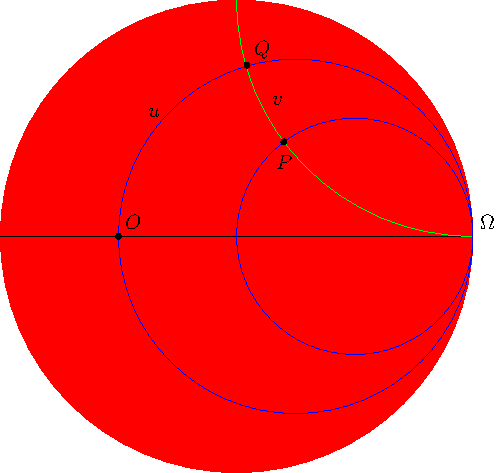
\includegraphics{images/11-horocyclebased}}
\caption{A horocycle-based coordinate system on the Poincaré disc. Blue curves represent horocycles tangent at ideal point $\Omega$, green lines depict perpendicular geodesics.}\label{fig:horocyclecoord}
\end{figure}

On the Poincaré disc $\mathcal{P}$, the coordinates of a point $P$ are denoted by $(u,v)$, where:
\begin{itemize}
\item $u$ represents the signed length of $OQ$
\item $v$ represents the signed length of $QP$
\item The sign conventions adhere to the right-hand rule and orientation relative to the ideal point $\Omega$
\end{itemize}

We equip this coordinate system with the inner product:
$$
\mathbf{a} \cdot \mathbf{b} = \begin{bmatrix} a_u & a_v \end{bmatrix} \begin{bmatrix} e^{-2v} & 0 \\ 0 & 1 \end{bmatrix} \begin{bmatrix} b_u \\ b_v \end{bmatrix}
$$

And the corresponding metric tensor:
$$
ds^2 = e^{-2v} du^2 + dv^2
$$

The Laplacian operator in this coordinate system is expressed as:
$$
\Delta = e^{2v} \frac{\partial^2}{{\partial u}^2} + \frac{\partial^2}{{\partial v}^2} - \frac{\partial}{\partial v}
$$

In this coordinate framework, we define an assignment:

\begin{equation}\label{eq:exmp2}
a = u e^{-v}
\end{equation}

\begin{theorem}\label{thm:exmp2}
The assignment $a$ defined by formula \eqref{eq:exmp2} satisfies the flow equation \eqref{eq:flow}.
\end{theorem}

\begin{proof}
We establish this result by demonstrating that examples 1 and 2 are equivalent through a Möbius transformation. Consider the complex representation of the upper half plane:
$$
z = x + yi
$$

The Möbius transformation mapping the upper half plane to the Poincaré disc is given by:
$$
z \mapsto \frac{z-i}{z+i}
$$

\begin{figure}[ht]
\centering
\resizebox{0.8\textwidth}{!}{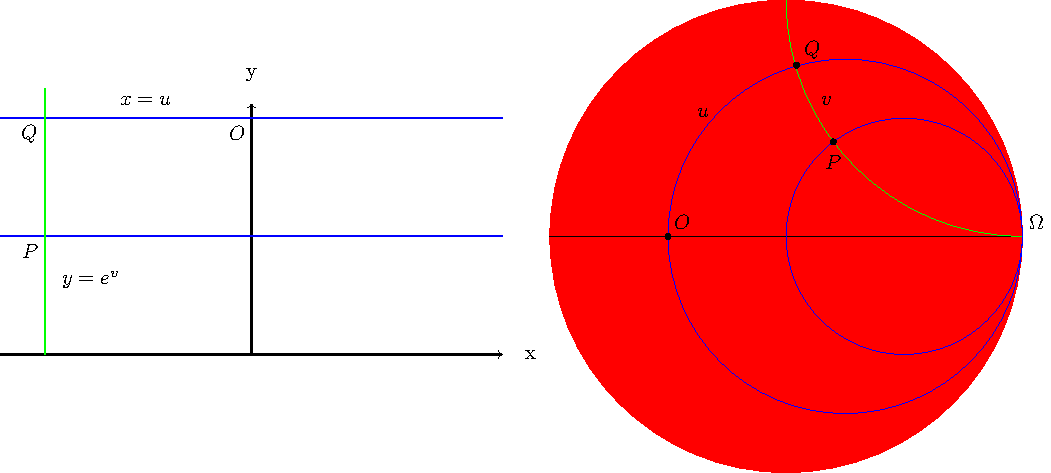
\includegraphics{images/12-proofbymapping}}
\caption{Mapping between the upper half plane and Poincaré disc models}\label{fig:mapping}
\end{figure}

This conformal transformation maps horizontal lines in $\mathcal{H}$ to horocycles sharing the ideal point $\Omega = 1$ in $\mathcal{P}$, and vertical geodesics in $\mathcal{H}$ to perpendicular geodesics in $\mathcal{P}$.

Expressed in the target coordinate system, this transformation yields:
$$
\begin{cases}
x = u\\
y = e^v \\
\end{cases}
$$

Substituting into the assignment from Example 1:
$$
a = -\frac{x}{y} = -\frac{u}{e^v} = -u e^{-v}
$$

Since the Möbius transformation is conformal and preserves the flow equation, and accounting for the orientation change, we obtain $a = u e^{-v}$ satisfying the flow equation.
\end{proof}

As in Example 1, we can verify that $a$ constitutes an eigenfunction of the Laplacian:
$$
\Delta a = e^{2v} \frac{\partial^2(u e^{-v})}{{\partial u}^2} + \frac{\partial^2(u e^{-v})}{{\partial v}^2} - \frac{\partial(u e^{-v})}{\partial v} = 2a
$$

These two examples, emerging from the same geometric foundation but expressed in different coordinate systems, demonstrate the fundamental properties of the first kind arithmetic expression space.

\subsection{Theoretical framework of $\mathfrak{E}_1$ space}\label{subsec:generalframework}

Building upon the foundational exemplars, we now establish a comprehensive theoretical framework for the first kind arithmetic expression space $\mathfrak{E}_1$. 

Consider the upper half plane $\mathcal{B}$:
$$
\{\mathcal{B}: (x, y) | y > 0 \}
$$

equipped with an inner product and metric tensor parameterized by constants $\mu$ and $\lambda$:

$$
\mathbf{a} \cdot \mathbf{b} = \begin{bmatrix} a_x & a_y \end{bmatrix} \begin{bmatrix} \frac{1}{\mu^2 y^2} & 0 \\ 0 & \frac{1}{\lambda^2 y^2} \end{bmatrix} \begin{bmatrix} b_x \\ b_y \end{bmatrix}
$$

$$
ds^2 = \frac{1}{y^2}\left(\frac{dx^2}{\mu^2} + \frac{dy^2}{\lambda^2}\right)
$$

The assignment function in this generalized framework maintains the form:

\begin{equation}\label{eq:genassignment}
a = - \frac{x}{y}
\end{equation}

This defines the first kind arithmetic expression space $\mathfrak{E}_1$, characterized by the following theorem:

\begin{theorem}\label{thm:generalE1}
The assignment $a$ given by \eqref{eq:genassignment} satisfies the flow equation \eqref{eq:flow} with parameters $\mu$ and $\lambda$, independent of the specific values of these generators.
\end{theorem}

\begin{proof}
The differential of the assignment is given by:
$$
da = d\left(-\frac{x}{y}\right) = \frac{xdy - ydx}{y^2} = -\frac{dx + a dy}{y}
$$

The differential of arc length is expressed as:
$$
ds = \frac{1}{y}\sqrt{\frac{dx^2}{\mu^2} + \frac{dy^2}{\lambda^2}}
$$

Therefore:
$$
\frac{da}{ds} = - \frac{dx + a dy}{y} \cdot \frac{y}{\sqrt{\frac{dx^2}{\mu^2} + \frac{dy^2}{\lambda^2}}} = -\frac{dx + a dy}{\sqrt{\frac{dx^2}{\mu^2} + \frac{dy^2}{\lambda^2}}}
$$

In the local coordinate system determined by $(-1, 0)$ and $(0, -1)$ according to the right-hand rule:

$$
\cos \theta = \frac{-\frac{dx}{\mu}}{\sqrt{\frac{dx^2}{\mu^2} + \frac{dy^2}{\lambda^2}}} \quad \text{and} \quad \sin \theta = \frac{-\frac{dy}{\lambda}}{\sqrt{\frac{dx^2}{\mu^2} + \frac{dy^2}{\lambda^2}}}
$$

Substituting these values:
$$
\frac{da}{ds} = \mu \cos \theta + a \lambda \sin \theta
$$

This precisely corresponds to the flow equation \eqref{eq:flow} with the given parameters $\mu$ and $\lambda$.
\end{proof}

The $\mathfrak{E}_1$ space is distinguished by its intrinsic connection to hyperbolic geometry and the property that the assignment function $a = -x/y$ constitutes an eigenfunction of the Laplacian operator with eigenvalue 2. This space provides a natural geometric framework for analyzing arithmetic expressions, particularly those involving addition and multiplication operations.

\subsection{Geometric propagation mechanisms}\label{subsec:geompropagation}

The flow equation in the $\mathfrak{E}_1$ space can be interpreted as describing the propagation of arithmetic expressions. This interpretation extends the propagation method discussed in Section \ref{subsec:propagation-method}.

In the $\mathfrak{E}_1$ space, paths along constant $x$ (vertical geodesics in the upper half plane) correspond to multiplication operations, while paths along constant $y$ (horizontal geodesics) correspond to addition operations. The assignment value $a = -x/y$ propagates according to the flow equation as we traverse these paths.

The propagation can be visualized as wavefronts emanating from source points in the upper half plane. Points with identical assignment values form equipotential curves, and the flow equation governs the geometric evolution of these wavefronts.

From equation \eqref{eq:gradevo5}, we recall that along the gradient direction ($\phi=0$) starting from $a_0=0$:
\begin{equation}
a = \pm \frac{\mu}{\lambda} \sinh(\lambda s)
\end{equation}

This expression exhibits a structural similarity to the formula for the circumference of a circle in hyperbolic space with curvature $-\lambda^2$:
\begin{equation}
C = \frac{2\pi}{\lambda} \sinh(\lambda s)
\end{equation}

This correspondence suggests that the assignment $a$ propagates analogously to expanding concentric circles in hyperbolic space, with the zero assignment locus serving as the collection of centroids from which these circles emanate.

The dual perspective of propagation and evaluation provides a powerful framework for understanding arithmetic expressions geometrically:
1. Evaluation of an expression follows geodesic paths through the $\mathfrak{E}_1$ space
2. Different evaluation orders correspond to distinct paths with identical endpoints
3. The flow equation ensures that the final value remains invariant with respect to the path taken (for evaluable expressions)

\subsection{Grid structures}\label{subsec:grids}

A significant geometric characteristic of the first kind arithmetic expression space is the presence of two distinct yet interrelated grid structures, each encoding addition and multiplication operations in different ways. These dual grids reflect the geometric structure of the Baumslag–Solitar group, whose Cayley graph exhibits an anisotropic, hierarchical lattice with a natural correspondence to mixed additive-multiplicative expressions.

Both grid structures are constructed within the upper half-plane model. The first grid is rectilinear, consisting of horizontal lines encoding addition operations and vertical lines encoding multiplication operations. Specifically, this grid is constructed through iterative applications of these two operations to generate a lattice in the $(x,y)$ coordinates. Each horizontal displacement from $(x,y)$ to $(x+1,y)$ represents an addition, and each vertical displacement from $(x,y)$ to $(x,2y)$ represents a multiplication by 2. The grid vertices correspond to values of expressions constructed from repeated applications of addition and multiplication operations, typically originating from a rational base point, often designated as 1.

Notably, in this first grid, the scalar field $a$ remains invariant under variations of the metric parameters $\mu$ and $\lambda$. That is, while the geometric properties of the space (lengths and angles) vary with these parameters, the locus where $a=0$—specifically, the vertical line $x=0$—remains structurally invariant and unaffected by changes in $\mu$ and $\lambda$.

The second grid emerges through a conformal transformation, specifically the Möbius transformation acting within the upper half-plane. This transformation maps horizontal lines to semicircles centered on the real axis and vertical rays to orthogonal semicircles. Under this transformation, the roles of addition and multiplication are effectively interchanged. The addition-multiplication structure of the first grid transforms into a new system of curved geodesics: the images of addition steps now follow curved trajectories around the origin, while the multiplicative steps exhibit contraction and inversion properties.

Although the visual structure of the second grid exhibits greater complexity, it retains a profound arithmetic coherence. The grid vertices continue to correspond to expressions generated through repeated applications of addition and multiplication operations, albeit composed under the transformed geometry. This grid demonstrates enhanced flexibility: under the conformal transformation, the images of zero lines such as $x=0$ are no longer fixed but deform into dynamic arcs. Consequently, the second grid accommodates a richer family of zero structures, allowing for the possibility of curved, branching, or nested nodal sets that vary with $\mu$, $\lambda$, or the choice of conformal framing.

Each of these grid structures can be interpreted as a geometric realization of a Cayley graph:

\begin{itemize}
\item The rectilinear grid corresponds to the Cayley graph of the Baumslag–Solitar group $BS(1,2)$, where multiplication by 2 followed by addition by 1 follows the relation $b^{-1}ab = a^2$.
\item The transformed (dual) grid corresponds to the Cayley graph of the dual Baumslag–Solitar group, where the roles of addition and multiplication are inverted.
\end{itemize}

Thus, the two grid systems exhibit duality not only in geometric terms but also in group-theoretic structure. The Möbius transformation, acting within the upper half-plane, connects these dual groups by exchanging generators and inverting flow directions, reflecting an intrinsic duality in the geometric composition of arithmetic operations.

The coexistence of these dual grid structures—one linear, one curved—linked via conformal symmetry, suggests a profound underlying symmetry in the geometry of arithmetic expressions. This duality reflects how different evaluation paths or expression embeddings can be interpreted as projections from a common, more complex geometric source. Understanding this symmetry may provide a pathway to expressing arithmetic relations via modular or automorphic structures, particularly in the context of recursive expressions and iterative identities, where Baumslag–Solitar-like behavior naturally emerges.

We conjecture that this grid duality corresponds to a deeper expression-theoretic equivalence, and that the Möbius transformation connecting them manifests an underlying arithmetic symmetry in expression geometry.

\subsection{Torsion under scale transformation}\label{subsec:gridsandtorsion}

The addition-multiplication grid introduced in Section~\ref{subsec:meshgrid} has a natural embedding in the arithmetic expression space $\mathfrak{E}_1$. This grid consists of two orthogonal families of curves:

\begin{enumerate}
\item \textbf{Addition curves} (blue lines): horizontal geodesics along which $y$ remains constant, representing iterated additions.
\item \textbf{Multiplication curves} (green lines): vertical or logarithmically scaled geodesics where the ratio $x/y$ remains constant, representing multiplicative transformations.
\end{enumerate}

This grid structure facilitates the geometric analysis of \emph{arithmetic torsion}—a quantity arising from the non-commutativity of certain additive and multiplicative expression sequences. Specifically, torsion quantifies the discrepancy between two seemingly equivalent but differently ordered expressions.

\begin{figure}[ht]
\centering
\resizebox{0.8\textwidth}{!}{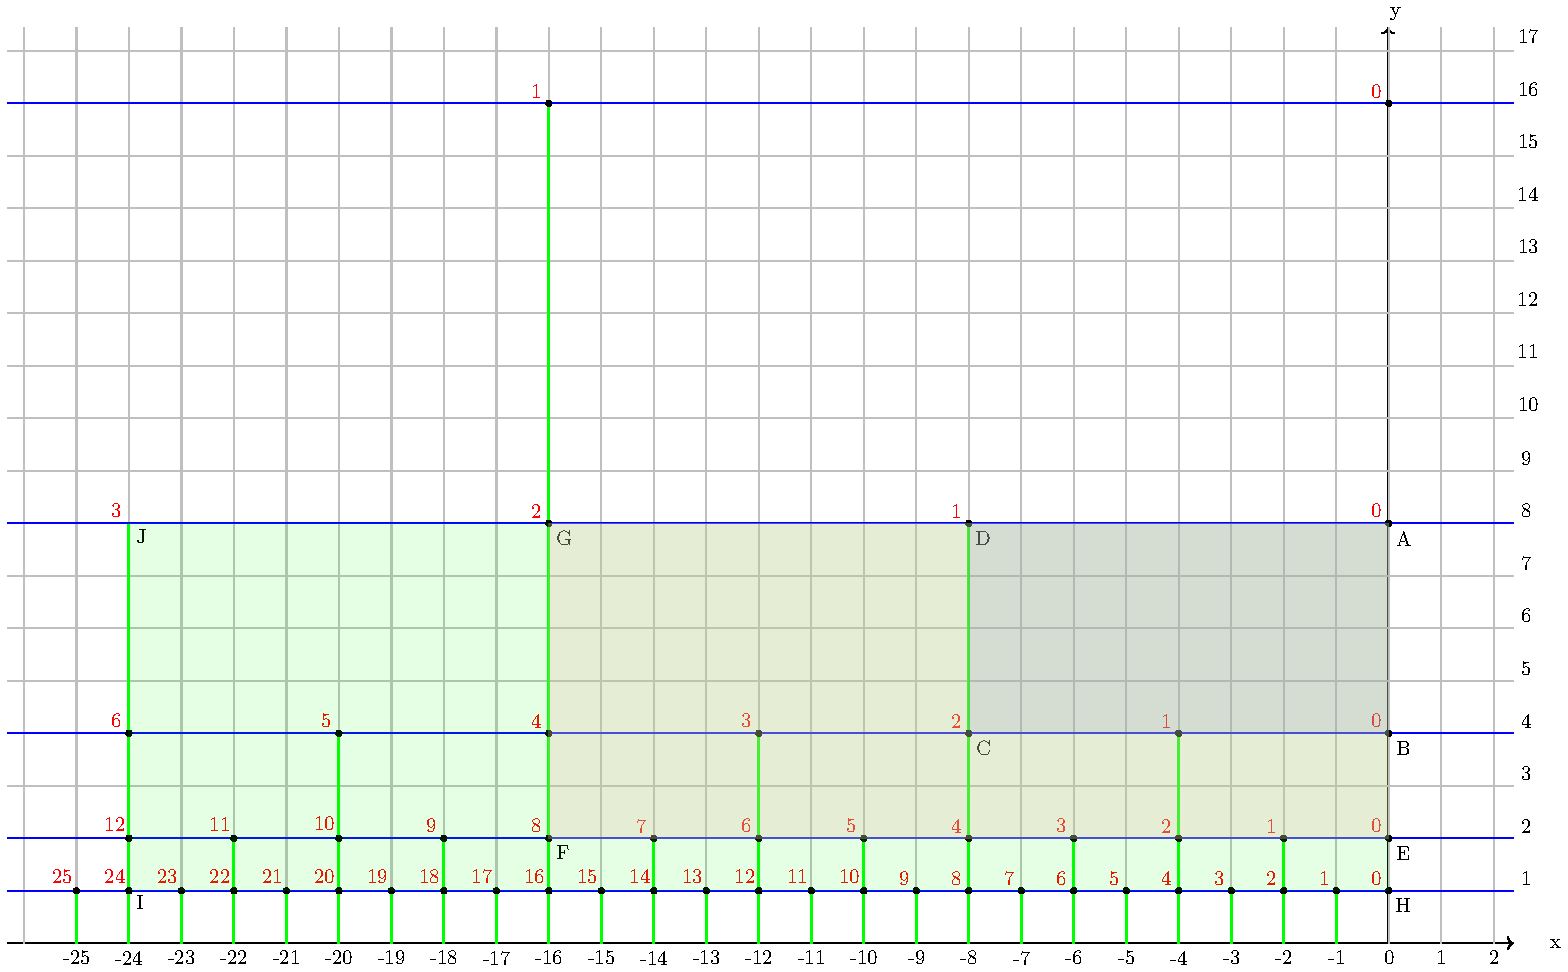
\includegraphics{images/17-area-formula}}
\caption{Illustration of the correspondence between hyperbolic area and arithmetic torsion}\label{fig:area-formula}
\end{figure}

Figure~\ref{fig:area-formula} illustrates the relationship between the area enclosed by expression paths in the grid and the resulting torsion. Consider the following expression identity comparisons:

\begin{itemize}
\item One-step case:
\begin{equation}
x \times 2 + 1 - (x + 1) \times 2 = -1
\end{equation}

\item Two-step case:
\begin{equation}
    x \times 4 + 2 - (x + 2) \times 4 = -6
\end{equation}

\item Three-step case:
\begin{equation}
    x \times 8 + 3 - (x + 3) \times 8 = -21
\end{equation}\end{itemize}

These differences correspond precisely to the hyperbolic areas enclosed between alternative evaluation paths:

\begin{itemize}
\item The region $ABCD$ encompasses 1 unit cell.
\item The region $AEFG$ encompasses 6 unit cells.
\item The region $AHIJ$ encompasses 21 unit cells.
\end{itemize}
Thus, arithmetic torsion accumulates proportionally to the area enclosed by the grid paths, indicating an intrinsic connection between algebraic non-commutativity and geometric surface area.

This relationship is expressed through a differential formulation:
\begin{equation}
d\tau = \mu \lambda\, du\, dv
\end{equation}

where $d\tau$ represents the infinitesimal arithmetic torsion, and $du\, dv$ denotes the area element in the $(u, v)$ coordinate system adapted to the grid.

The analogy with curvature in differential geometry becomes evident: just as Gaussian curvature encodes deviation from flatness, arithmetic torsion quantifies deviation from commutativity in arithmetic flow. In this sense, torsion constitutes a measure of the operational significance of evaluation order.

The $\mathfrak{E}_1$ space thus provides a mathematical framework where algebraic non-commutativity manifests as measurable geometric distortion—establishing a novel interpretation of arithmetic structure as a form of discrete curvature. This opens avenues for investigating further geometric invariants such as torsion density, torsion-induced flow bifurcation, and potentially a Gauss–Bonnet-type integral identity for arithmetic surfaces.


\subsection{Tube structure}\label{sec:tubestructure}

In preceding sections, we introduced the expression space $\mathfrak{E}_1$ as a geometric realization of arithmetic flow under fixed generator parameters $\mu$ and $\lambda$. However, more complex structures emerge when we consider the family of all such spaces parameterized by $\lambda$ (or both parameters) and analyze the behavior of expressions across this family. This leads naturally to the concept of a \emph{tube structure}.

\subsubsection{From slices to parametric families}

Each individual $\mathfrak{E}_1$ space may be conceptualized as a single "slice" within a parameterized family of expression spaces indexed by $\lambda$. Within each slice, arithmetic expressions are realized as geodesic paths, their evaluations governed by the scalar field $a$, and their flow by the local metric tensor.

Consider fixing an expression—for example, a polynomial of the form $P(x)$—and examining how its geometric representation evolves as $\lambda$ varies. This defines a \emph{fiber} that traverses through the slices of $\mathfrak{E}_1$ spaces, delineating a trajectory across a higher-dimensional space. The totality of such fibers over all values of $\lambda$ constitutes a new structure: a \emph{tube}.

\subsubsection{Tube structure as total space}

We define a \textbf{tube structure} $\mathcal{T}$ as the total space formed by the disjoint union of a continuous family of $\mathfrak{E}_1$ spaces:
\begin{equation}
\mathcal{T} = \bigsqcup_{\lambda > 0} \mathfrak{E}_1^{(\lambda)}
\end{equation}
endowed with a topology and bundle-like structure facilitating coherent traversal along the $\lambda$-direction.

In this structure:
\begin{itemize}
\item The base space is the parameter domain $\Lambda$ (e.g., $\mathbb{R}^+$).
\item Each fiber over $\lambda$ is a geometric expression space $\mathfrak{E}_1^{(\lambda)}$.
\item Expression paths can be lifted to continuous trajectories across fibers.
\item Polynomials $P(x)$, viewed as expressions in $\mathfrak{E}_1$, trace canonical sections through $\mathcal{T}$.
\end{itemize}

\subsubsection{Zero surfaces and nodal evolution}

A primary motivation for examining tube structures is to investigate how \emph{zero lines}—loci where an expression evaluates to zero—evolve across $\lambda$. In a single $\mathfrak{E}_1$ slice, these constitute 1-dimensional curves. As $\lambda$ varies, their union forms a 2-dimensional surface within $\mathcal{T}$, which we designate as a \emph{zero surface}.

These zero surfaces may exhibit several notable phenomena:
\begin{itemize}
\item \textbf{Bifurcation}: new zero lines may emerge or merge as $\lambda$ undergoes variation.
\item \textbf{Branching}: certain expressions may exhibit multi-valued zero loci across $\lambda$.
\item \textbf{Topology change}: zero surfaces may develop handles, pinch points, or singularities.
\end{itemize}

This perspective enables sophisticated analysis of expression dynamics—particularly when considering a family of expressions or differential equations involving $\lambda$.

\subsubsection{Canonical polynomials as fibers}

In practical applications, we frequently analyze a fixed expression such as a polynomial $P(x)$, evaluating it at $x=e^\lambda$. This yields a one-parameter family of values:
\begin{equation}
P(e^\lambda), \quad \lambda \in \mathbb{R}
\end{equation}
Each evaluation corresponds to a point in a fiber $\mathfrak{E}_1^{(\lambda)}$, and the totality defines a canonical section in the tube structure.

More generally, expressions involving both $x$ and $\lambda$ naturally trace \emph{embedded submanifolds} within $\mathcal{T}$. These can be utilized to analyze asymptotic behavior, resonance patterns, or nodal crossings across a family of arithmetic flows.

The tube structure formalism facilitates multiple investigative approaches:

\begin{itemize}
\item Examining global properties of zero surfaces (e.g., genus, curvature concentration)
\item Constructing flow equations across $\lambda$-families, potentially defining connections or transport laws
\item Defining moduli of expression geometries as structured bundles over parameter spaces
\end{itemize}

Ultimately, tube structures provide a mathematical framework in which arithmetic expression dynamics can be analyzed analogously to field theory, with expressions acting as structured sections and torsion/curvature defining local invariants.
